\subsection{Multinomial Logistic Regression}

Ta sử dụng một mạng Multi Layer Perceptron có 1 lớp ẩn, lớp ẩn gồm 64 neuron.
Ta chỉ sử dụng vector đầu vào là vector gốc ban đầu

\subsubsection{Mô hình cho tập dữ liệu chỉ bao gồm các quan sát có cột "emailtotal" không phải giá trị null}

Ta có bảng kết quả huấn luyện mô hình:

\begin{python}
                    precision    recall  f1-score   support

   Keeping house       0.00      0.00      0.00        58
           Other       0.00      0.00      0.00         8
         Retired       0.17      0.08      0.11       109
          School       0.00      0.00      0.00        14
Temp not working       0.00      0.00      0.00        15
Unempl, laid off       0.00      0.00      0.00        25
Working fulltime       0.54      0.93      0.68       351
Working parttime       0.00      0.00      0.00        80

        accuracy                           0.51       660
       macro avg       0.09      0.13      0.10       660
    weighted avg       0.31      0.51      0.38       660
\end{python}

và ma trận nhầm lẫn:

\begin{figure}[H]
    \centering
    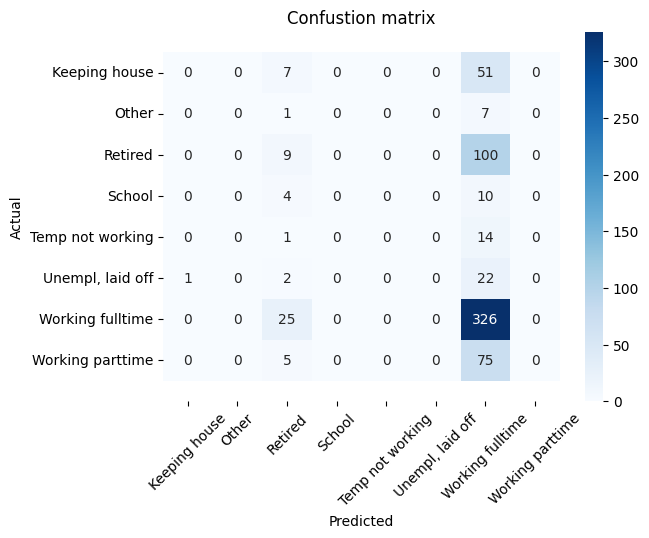
\includegraphics[width=0.6\textwidth]{figures/Thanh/Models/MLP_Deep_Learning/Non_null_models_confusion_matrix_MLP_original_features.png}
    \caption{Ma trận nhầm lẫn của mô hình MLP khi vector đầu vào là vector gốc ban đầu}
    \label{fig:Non_null_models_confusion_matrix_MLP_original_features}
\end{figure}

Tuy mô hình deep learning được đánh giá có khả năng phân loại dữ liệu tốt nhưng ta nhận thấy kết quả phân loại không khác biệt hay nổi trội hơn các mô hình trước.
Điều này càng phản ánh sự trỗn lẫn, khó phân biệt của phân phối dữ liệu tương ứng với từng nhãn trong cột wrkstat.